\subsection{Glyph: \glyph{Omitted process}}
\label{sec:omitted}

Omitted processes are processes that are known to exist, but are omitted from the map for the sake of clarity or parsimony. A single \glyph{omitted process} can represent any number of actual processes. The \glyph{omitted process} is different from a \glyph{submap}. While a \glyph{submap} references to an explicit content, that is hidden in the main map, the \glyph{omitted process} does not ``hide'' anything within the context of the map, and cannot be ``unfolded''.

\begin{glyphDescription}

\glyphSboTerm
SBO:0000397 ! omitted process


\glyphIncoming
One or more \glyph{consumption} arcs (\sect{consumption})\footnote{Zero \glyph{consumption arcs} are allowed in the case of a reversible process.}, zero or more \glyph{modulation} arcs (\sect{modulations}).



\glyphOutgoing
One or more \glyph{production} arcs (\sect{production}).


\glyphContainer
An \glyph{omitted process} is represented by a square shape that contains two parallel slanted lines oriented northwest-to-southeast and separated by an empty space.
The shape is linked to two ports, that are small arcs attached to the centres of opposite sides of the shape, as shown in \fig{omitted}.
The incoming \glyph{consumption} (\sect{consumption}) and outgoing \glyph{production} (\sect{production}) arcs are linked to the extremities of those ports.

The \glyph{modulation arcs} (\sect{modulations}) point to the other two sides of the shape.

\glyphLabel
None.

\glyphAux
None.

\end{glyphDescription}

\begin{figure}[H]
  \centering
  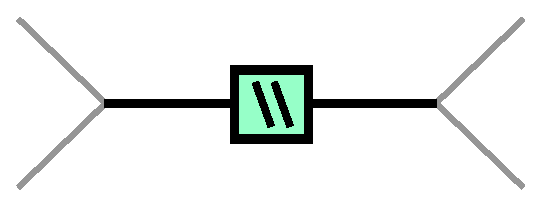
\includegraphics{images/omitted}
  \caption{The \PD glyph for \glyph{omitted process}.}
  \label{fig:omitted}
\end{figure}
